\documentclass{lmcs} %%% last changed 2014-08-20

%% mandatory lists of keywords
\keywords{BPMN, Higher-order model transformation, Graph transformation, Model checking, Formalization}
% My packages
% Footnotes inside tables
\usepackage{footnote}
\usepackage{csquotes} % enquote command
\usepackage{threeparttable} % Tables with notes
\makesavenoteenv{tabular}
\makesavenoteenv{table}
% Listings
\usepackage{courier} %% Sets font for listing as Courier.
\usepackage{listings, xcolor}
\definecolor{javared}{rgb}{0.6,0,0} % for strings
\definecolor{javagreen}{rgb}{0.25,0.5,0.35} % comments
\definecolor{javapurple}{rgb}{0.5,0,0.35} % keywords
\definecolor{javadocblue}{rgb}{0.25,0.35,0.75} % javadoc
 
\lstset{language=Java,
basicstyle=\ttfamily,
keywordstyle=\color{javapurple}\bfseries,
stringstyle=\color{javared},
commentstyle=\color{javagreen},
morecomment=[s][\color{javadocblue}]{/**}{*/},
numbers=left,
numberstyle=\tiny\color{black},
stepnumber=2,
numbersep=10pt,
tabsize=4,
showspaces=false,
showstringspaces=false}

\definecolor{gray}{rgb}{0.4,0.4,0.4}
\definecolor{darkblue}{rgb}{0.0,0.0,0.6}
\definecolor{cyan}{rgb}{0.0,0.6,0.6}

\lstdefinelanguage{XML}
{
  morestring=[b]",
  morestring=[s]{>}{<},
  morecomment=[s]{<?}{?>},
  moredelim=[s][\color{darkblue}]{<}{\ },
  moredelim=[s][\color{darkblue}]{</}{>},
  moredelim=[l][\color{darkblue}]{/>},
  moredelim=[l][\color{darkblue}]{>},
  stringstyle=\color{black},
  identifierstyle=\color{darkblue},
  keywordstyle=\color{cyan},
  morekeywords={id,sourceRef,targetRef, processSnapshot}% list your attributes here
}
% My packages end

\usepackage{hyperref}

\begin{document}

\title[Formalization and analysis of BPMN using graph transformation systems]{A higher-order transformation approach to the formalization and analysis of BPMN using graph transformation systems\rsuper*}
\titlecomment{{\lsuper*}This article is an extended version of \cite{krauterFormalizationAnalysisBPMN2023}}
% \thanks{thanks, optional.}	%optional

\author[T.~Kr\"{a}uter]{Tim Kr\"{a}uter\lmcsorcid{0000-0003-1795-0611}}[a]
\author[A.~Rutle]{Adrian Rutle\lmcsorcid{0000-0002-4158-1644}}[a]
\author[H.~K\"{o}nig]{Harald K\"{o}nig\lmcsorcid{0000-0001-6304-6311}}[a,b]
\author[Y.~Lamo]{Yngve Lamo\lmcsorcid{0000-0001-9196-1779}}[a]

\address{Western Norway University of Applied Sciences, Bergen, Norway}
\email{tkra@hvl.no, aru@hvl.no, hkoe@hvl.no, yla@hvl.no}

\address{University of Applied Sciences, FHDW, Hanover, Germany}
\email{harald.koenig@fhdw.de}

\begin{abstract}
  \noindent
The Business Process Modeling Notation (BPMN) is a widely used standard notation for defining intra- and inter-organizational workflows.
However, the informal description of the BPMN execution semantics leads to different interpretations of BPMN elements and difficulties in checking behavioral properties.
In this article, we propose a formalization of the execution semantics of BPMN that, compared to existing approaches, covers more BPMN elements while also facilitating property checking.
Our approach is based on a higher-order transformation from BPMN models to graph transformation systems.
As proof of concept, we provide an implementation of our approach as an open-source web-based tool. 
\end{abstract}

\maketitle
\section{Introduction}
In today's fast-paced business environment, organizations with complex workflows require a powerful means to accurately map, analyze, and optimize their processes. 
Business Process Modeling Notation (BPMN) \cite{objectmanagementgroupBusinessProcessModel2013} is a widely used standard to define these workflows.
However, the informal description of the BPMN execution semantics leads to different interpretations of BPMN models and difficulties in checking behavioral properties \cite{corradiniFormalApproachAnalysis2021}.
Various studies have shown that business process models suffer from control-flow errors \cite{mendlingEmpiricalStudiesProcess2009}.
Formalizing BPMN would drastically reduce the cost of business process automation by facilitating the detection of errors and optimization potentials in process models already during design time.
To this end, we propose a formalization that covers most of the BPMN elements used in practice and, in addition, supports checking behavioral properties.
General behavioral properties such as \textit{Safeness} and \textit{Soundness} were adapted to BPMN in \cite{corradiniClassificationBPMNCollaborations2018}. They can uncover potential flaws in BPMN models leading to deadlocks or other undesirable execution states.

In this article, we consider two fundamental concepts when formalizing the execution semantics of BPMN.
First, \textit{state structure}, i.e., how model instances are represented during execution.
The state structure corresponds to the type graph in Graph Transformation (GT) systems.
Second, \textit{state-changing elements}, i.e., which elements in a model encode state changes.
These elements are implemented using GT rules, which we automatically generate based on a Higher-Order model Transformation (HOT) \cite{tisiUseHigherOrderModel2009} for each specific BPMN model, as shown in \autoref{fig:approach}.

\begin{figure}[ht]
    \centering
    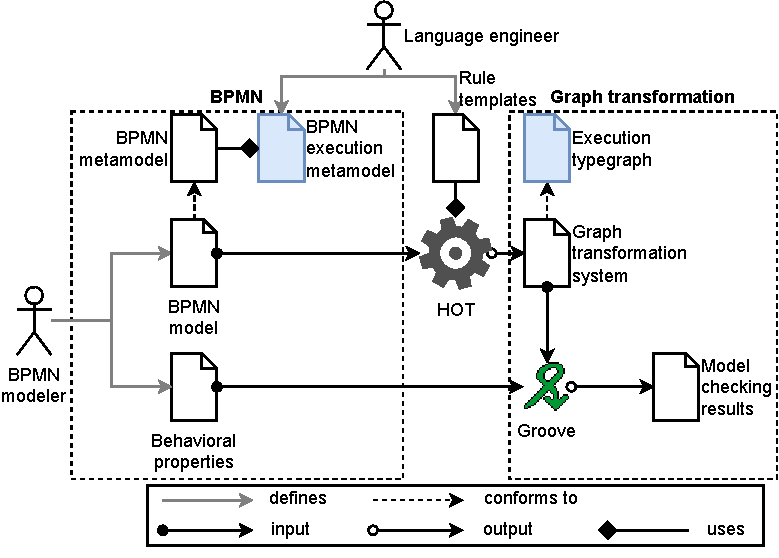
\includegraphics[width=0.85\textwidth]{images/bpmn_semantics-overview.pdf}
    \caption{Overview of the approach}
    \label{fig:approach}
\end{figure}

To begin the BPMN modeling process, a modeler first defines the BPMN model. 
The BMPN model may be checked against a predefined list of general behavioral properties, such as safeness and soundness.
Furthermore, the modeler may also define custom behavioral properties specifically defined for the BPMN model.
%To begin the BPMN modeling process, a modeler first defines the BPMN model and its corresponding behavioral properties for evaluation.
%He can also define atomic propositions for his BPMN model if he defines custom behavioral properties besides checking general BPMN properties.
The defined BPMN model must adhere to the BPMN metamodel as outlined in the BPMN specification by the Object Management Group \cite{objectmanagementgroupBusinessProcessModel2013}.
The BPMN execution metamodel is defined by language engineers, utilizing the BPMN metamodel as a foundation to create the state structure for executing BPMN models. 
%To create the state structure for BPMN, the BPMN execution metamodel is defined by language engineers, utilizing the BPMN metamodel as a foundation.
%Typically, an execution metamodel is created by extending the languages metamodel.



We define a HOT from BPMN models to GT systems.
We call the transformation \textit{higher-order} since the resulting graph-transformation systems represent model-transformations themselves \cite{tisiUseHigherOrderModel2009}.
The HOT creates a GT system, i.e., GT rules and a start graph for a given BPMN model.
It is defined using rule generation templates, which describe how GT rules should be generated for each state-changing element in BPMN (see \autoref{sec:formalization}).
The obtained GT system conforms to the execution type graph, which corresponds to the BPMN execution metamodel.
In the figure, we have colored both artifacts blue to visualize that they contain the same information.
Ultimately, we use Groove as an execution engine for the GT system and to check the behavioral properties defined earlier.
To facilitate model checking of custom behavioral properties, we create specific GT rules for the constituent atomic propositions during the HOT.
%Atomic propositions are converted to specific GT rules for Groove during the HOT to facilitate model checking of custom behavioral properties.

%Our approach has been implemented in
We provide an implementation of our approach as a user-friendly, open-source web-based tool, the \textit{BPMN Analyzer}, which can be used online without needing installation \cite{timkrauterLMCS2024Artifacts2023}.
%%The BPMN Analyzer was validated using a comprehensive test suite.
%Additionally, our approach is versatile as it can be applied to formalize other behavioral languages, such as activity diagrams, state charts, and more.
%To define the execution semantics of a different behavioral language, one simply needs to establish a new execution metamodel and HOT (see the language engineer in \autoref{fig:approach}).
The overview in \autoref{fig:approach} is divided into two separated parts, denoted by dashed rectangles, to indicate the versatility of the approach as it can be applied to formalize other behavioral languages, such as activity diagrams and state charts. %cite?
This formalization will require the language engineer to establish a new execution metamodel and a HOT for the new language.


% Contributions summary
The contribution of this article is twofold.
First, we introduce a new approach utilizing a HOT to generate GT rules --- instead of providing fixed model-independent GT rules --- to formalize the semantics of a behavioral language.
Second, we apply our approach to BPMN, resulting in a formalization covering most BPMN elements that supports behavioral property checking.

% Compared to the conference version
This article extends \cite{krauterFormalizationAnalysisBPMN2023} as follows.
% BPMN semantics formalization: More elements/features described
(i) We explain many more BPMN elements, which are covered by our approach (see elements highlighted in blue in \autoref{fig:bpmnelementsOverview}).
% Model checking: Custom properties
(ii) We enhance the explanation of the custom properties in \autoref{sec:modelChecking} by using an order handling example process to illustrate use cases for these properties.
% Implementation: Custom properties editor and new three-step flow
(iii) We detail the extensively improved BPMN analyzer tool in \autoref{sec:impl} in which modelers may use our new atomic proposition editor. %, which is created based on our concrete syntax for describing snapshots of processes.
% Scalability
(iv) We test the scalability of our approach with 300 synthetically generated BPMN models of various sizes in \autoref{sec:scalability}. 

% Article outline
\textbf{Outline} The remainder of this article is structured as follows.
First, in \autoref{sec:preliminaries}, we introduce BPMN and briefly explain the theoretical background of our contribution.
Second, we describe the BPMN semantics formalization using the HOT (\autoref{sec:formalization}) before explaining how this can be utilized for model checking general BPMN and custom properties (\autoref{sec:modelChecking}).
Then, we detail the BPMN Analyzer tool in \autoref{sec:impl} and we describe how we tested the scalability of our approach in \autoref{sec:scalability}.
Finally, we discuss related work regarding BPMN element coverage in \autoref{sec:relatedWork} and conclude in \autoref{sec:conclusion}.

\section{Preliminaries} \label{sec:preliminaries}

In this section, we briefly introduce the execution semantics of BPMN, and readers are encouraged to consult \cite{freundRealLifeBPMNUsing2019} or the BPMN specification \cite{objectmanagementgroupBusinessProcessModel2013} for more in-depth information. 
Furthermore, we outline our application of GTs to formalize the execution semantics of BPMN.
Finally, we provide a brief overview of the theoretical principles that underlie our use of GTs.


\subsection{BPMN}
% \autoref{fig:bpmnMetamodel} depicts the structure of BPMN models with the corresponding concrete syntax BPMN symbols contained in clouds.
% A BPMN model is represented by a \textsf{Collaboration} that has \textsf{participants} and \textsf{messageFlows} between \textsf{InteractionNode}s.
% Each participant is a \textsf{Process} containing \textsf{flowNodes} connected by \textsf{SequenceFlow}s.
% A \textsf{FlowNode} is either an \textsf{Activity}, \textsf{Gateway}, or \textsf{Event}.
% Many types of \textsf{Activities}, \textsf{Gateways}, and \textsf{Events} exist.
\autoref{fig:bpmnMetamodel} depicts the structure of BPMN models with the corresponding concrete syntax BPMN symbols contained in clouds.
A BPMN model is represented by a \textsf{Collaboration} that has participant \textsf{Process}es and \textsf{MessageFlow}s between \textsf{InteractionNode}s.
Each participant is a \textsf{Process} containing \textsf{FlowNode}s connected by \textsf{SequenceFlow}s.
A \textsf{FlowNode} is either an \textsf{Activity}, \textsf{Gateway}, or \textsf{Event}.
Many types of activities, gateways, and events exist, such as send tasks, parallel gateways, and start events.
Activities represent certain tasks to be carried out during a process, while events may happen during the execution of these tasks.
Furthermore, gateways model conditions, parallelizations, and synchronizations \cite{freundRealLifeBPMNUsing2019}.

\begin{figure}[ht]
  \centering
  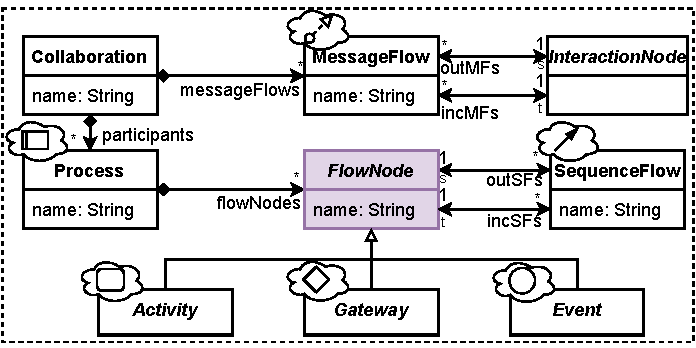
\includegraphics[width=0.9\linewidth]{images/bpmn_semantics-bpmn-metamodel.pdf}
  \caption{Excerpt of the BPMN metamodel \cite{objectmanagementgroupBusinessProcessModel2013}}
  \label{fig:bpmnMetamodel}
\end{figure}
% Containment: participants, messageFlows see fig. 9.33 in the BPMN spec.
% Containment: flowNodes (Process is FlowElementsContainer fig. 8.23). FlowElementsContainer has a containment of flow elements (also includes sequence flows)

The BPMN execution semantics is described using the concept of \textit{tokens} \cite{objectmanagementgroupBusinessProcessModel2013}, which can be located at sequence flows and specific flow nodes.
Tokens are consumed and created by flow nodes according to the connected sequence flows.
The \textsf{FlowNode} is colored purple in \autoref{fig:bpmnMetamodel} since it represents the \textit{state-changing elements} of BPMN, as described in \autoref{sec:formalization}.

A BPMN process is triggered by one of its start events, leading to a token at each outgoing flow of the triggered start event.
% Activities
Activities can start when at least one token is on an incoming sequence flow.
The start of an activity will move the incoming token to the activity.
When an activity terminates, it deletes its token and adds one at each outgoing sequence flow.
% Gateways
Furthermore, different gateway types exist, such as parallel and exclusive gateways.
Parallel gateways represent forks and joins, meaning they delete one token for each incoming sequence flow and add one token for each outgoing sequence flow.
Exclusive gateways represent an XOR by deleting a token from one incoming sequence flow and adding a token to exactly one of the outgoing sequence flows.
% Events (basic)
Events delete and add tokens similar to activities but have additional semantics depending on their type.
For example, message events will add or delete messages.

\subsection{Theoretical background}
We use typed attributed graphs to formalize the BPMN execution semantics.
Each state, i.e., token distribution during the execution of a BPMN model, is represented as an attributed graph typed by the BPMN execution type graph, which we introduce in \autoref{sec:formalization}.

Regarding GT, we utilize the single-pushout (SPO) approach with negative application conditions (NAC) \cite{ehrigALGEBRAICAPPROACHESGRAPH1997}, as implemented in Groove \cite{rensinkGROOVESimulatorTool2004}.
In addition, we utilize \textit{nested rules} with quantification to make parts of a rule repeatedly applicable or optional \cite{rensinkNestedQuantificationGraph2006,rensinkHowMuchAre2017}.
Moreover, we utilize the NACs to implement more intricate parts in the BPMN execution semantics, such as the termination of processes.

Formal definitions of SPO rules, their application, and the corresponding extensions of the theory (NACs, nested rules) are well-known, see \cite{ehrigALGEBRAICAPPROACHESGRAPH1997,rensinkNestedQuantificationGraph2006}.
We do not repeat them and instead focus on our practical contribution.


\section{BPMN semantics formalization} \label{sec:formalization}

The approach supports all the BPMN elements depicted in \autoref{fig:bpmnelementsOverview}.
These BPMN elements are divided into \textsf{Events}, \textsf{Gateways}, \textsf{Activities}, and \textsf{Edges}.
\textsf{Events} and \textsf{Activities} are further divided into subgroups.
Although all these elements have been implemented and tested (see \cite{timkrauterLMCS2024Artifacts2023}), we only explain the realization of the elements marked with a blue background due to space limitations.
In the following, first, we define the BPMN execution metamodel to represent the BPMN state structure, and then we explain our formalization of the elements in \autoref{fig:bpmnelementsOverview}.


\begin{figure}[ht]
    \centering
    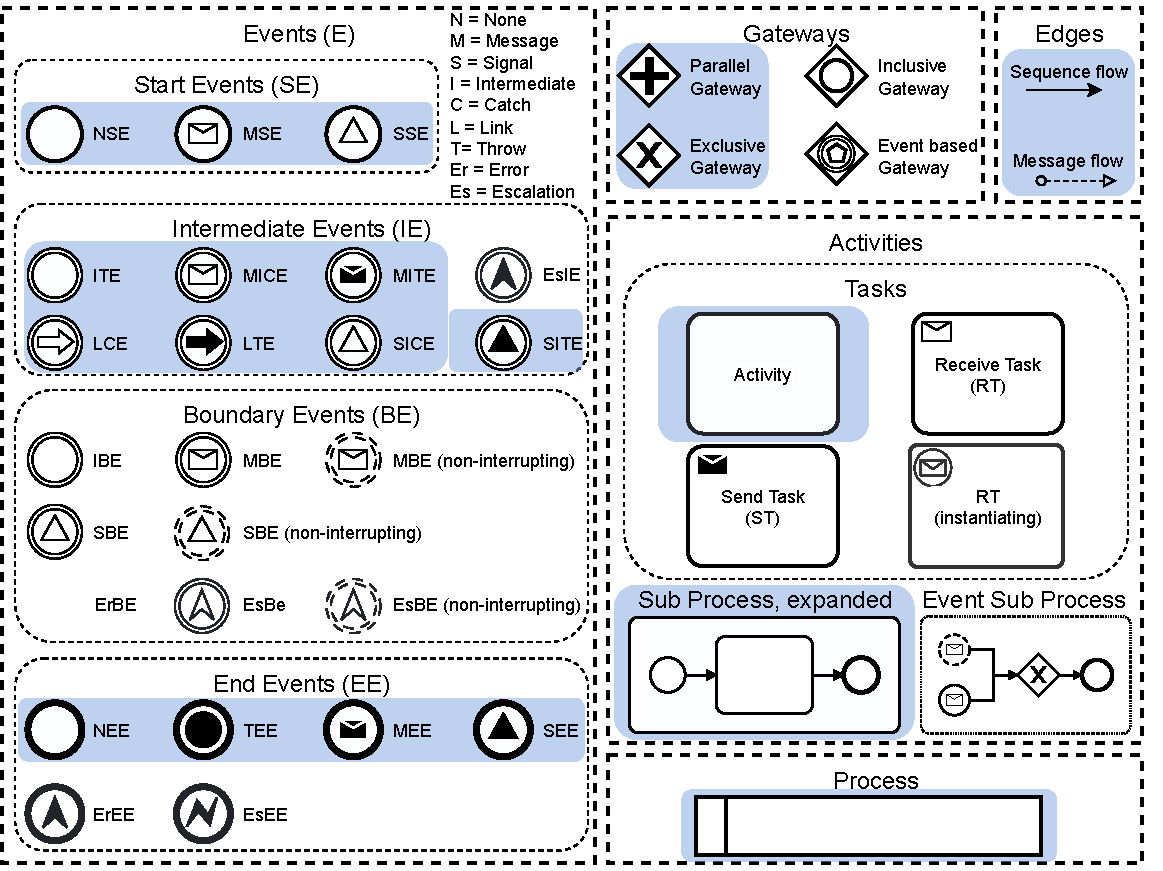
\includegraphics[width=0.99\textwidth]{images/bpmn_semantics-elements-overview.pdf}
    \caption{Overview of the supported BPMN elements (structure adapted from \cite{houhouFirstOrderLogicVerification2022})}
    \label{fig:bpmnelementsOverview}
\end{figure}


\subsection{BPMN execution metamodel}

In our formalization of BPMN, we utilize a token-based representation of the execution semantics, similar to the explanation in the informal description of the BPMN specification \cite{objectmanagementgroupBusinessProcessModel2013}.
To describe processes holding tokens during execution, we define the execution metamodel shown in \autoref{fig:bpmnExecutionMetamodel}, depicted as a UML class diagram.
The first task of a language engineer in our approach is to define the execution metamodel (see \autoref{fig:approach}).

\begin{figure}[ht]
  \centering
  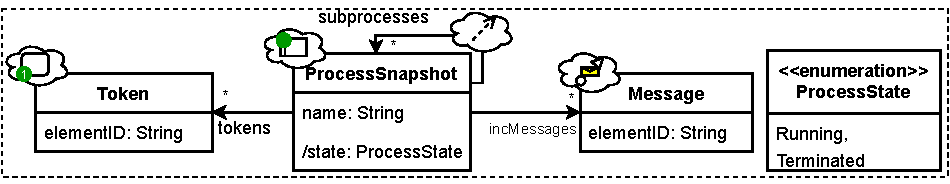
\includegraphics[width=1\linewidth]{images/bpmn_semantics-typegraph.pdf}
  \caption{BPMN execution metamodel}
  \label{fig:bpmnExecutionMetamodel}
\end{figure}

We use \textsf{ProcessSnapshot} to denote a running BPMN process with a specific token distribution that describes one state in the history of the process execution.
Every \textsf{ProcessSnapshot} has a set of \textsf{tokens}, incoming \textsf{messages}, and \textsf{subprocesses}.
A \textsf{ProcessSnapshot} has the state \textsf{Terminated} if it has no \textsf{tokens} or \textsf{subprocesses}.
Otherwise, it has the state \textsf{Running}.
A \textsf{Token} has an \textsf{elementID}, which points to the BPMN \textsf{Activity} or the \textsf{SequenceFlow} at which it is located.
A \textsf{Message} has an \textsf{elementID} pointing to a \textsf{MessageFlow}.
To concisely depict graphs conforming to this type graph, we introduce a concrete syntax in the clouds attached to the elements.
Our concrete syntax extends the BPMN syntax by adding process snapshots, subprocess relations, tokens, and messages.
Tokens are represented as colored circles drawn at their specified positions in a model.
In addition, we use colored circles at the top left of the bounding box, representing instances of the BPMN \textsf{Process}; these circles represent process snapshots.
The token's color must match the color of the process snapshot holding the token.
The concrete syntax was inspired by the bpmn-js-token-simulation \cite{camundaservicesgmbhBpmnjsTokenSimulation2023}.

Our BPMN execution metamodel was not created by extending the BPMN metamodel and adding missing concepts such as tokens and messages.
We chose to create a minimal execution model only containing concepts needed during execution.
This is only possible since the HOT generates our rules for each specific BPMN model such that the structure of each model is already implicitly encoded in the rules.
This design choice leads to smaller states in the GT system when compared to an execution metamodel that extends the BPMN metamodel.

The execution metamodel in \autoref{fig:bpmnExecutionMetamodel} is a UML class diagram without operations, which can be seen as an attributed type graph \cite{heckelGraphTransformationSoftware2020}.
We keep the execution metamodel and the execution type graph separate (see \autoref{fig:approach}) because the execution metamodel should be independent of the formalism used to define the execution semantics.
One can reuse the execution metamodel when changing the formalism or concrete tool implementing the formalism (in our case, Groove) by adjusting how the execution metamodel is transformed.
Using the execution metamodel as the type graph, we can now define how the start graph and GT rules for the different BPMN elements are created.

Since our approach is based on a HOT from BPMN to GT systems, we generate a \textit{start graph} and \textit{GT rules} for each given BPMN model (see \autoref{fig:approach}).
Generating the start graph for a BPMN model is straightforward.
First, for each process in the BPMN model, we generate a process snapshot if the process contains a \textit{none start event} (NSE).
An NSE describes a start event without a trigger (none).
Then, for each NSE, we add one token to each outgoing sequence flow.
An example of a start graph is shown in \autoref{fig:startGraph} using abstract and concrete syntax.

\begin{figure}[ht]
    \centering
    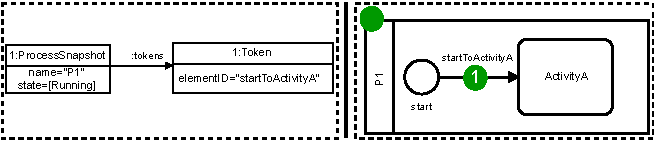
\includegraphics[width=0.85\textwidth]{images/startGraph.pdf}
    \caption{Example start graph in abstract (left) and concrete syntax (right)}
    \label{fig:startGraph}
\end{figure}

The HOT generates one or more GT rules for each \textsf{FlowNode}, i.e., state-changing element in a BPMN model.
In order to provide a better understanding of the transformation process, we will begin by presenting example results, namely the generated rules for an activity.
Following this, we will delve into an explanation of how our HOT creates these rules as well as rules for the other elements in \autoref{fig:bpmnelementsOverview}.

\autoref{fig:gtRuleAbstract} depicts an example GT rule ($L \to R$) to start an activity in abstract syntax.
The rule is straightforward: it moves a token from the incoming sequence flow to the activity.

\begin{figure}[ht]
    \centering
  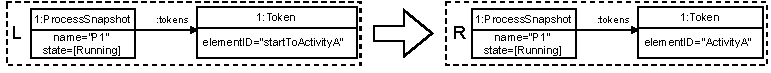
\includegraphics[width=1\textwidth]{images/rule_abstract.pdf}
  \caption{Example GT rule to start an activity (abstract syntax)}  \label{fig:gtRuleAbstract}
\end{figure}

For the rest of the article, we will depict all rules in the concrete syntax introduced earlier.
The rule from \autoref{fig:gtRuleAbstract} depicted in concrete syntax is shown on the left in \autoref{fig:gtRuleConcrete}.
The rule on the right in \autoref{fig:gtRuleConcrete} implements the termination of an activity, which will move one token from the activity to the outgoing sequence flow.

\begin{figure}[ht]
    \centering
  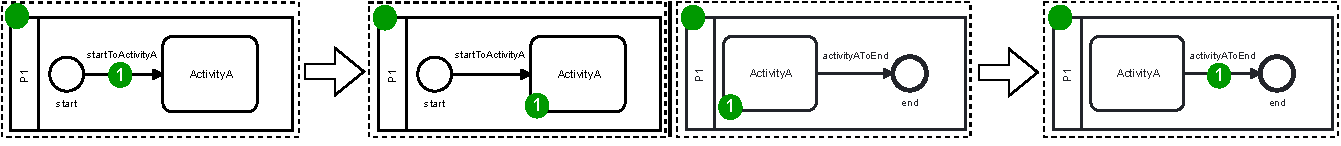
\includegraphics[width=1\textwidth]{images/rule_concrete.pdf}
  \caption{Example GT rules to start (left) and terminate (right) an activity}
  \label{fig:gtRuleConcrete}
\end{figure}

In the following subsections, we use our concrete syntax to define how our HOT generates these rules and rules for other flow nodes.
Elements of the HOT are depicted using rule generation templates that show how specific rules are created for various flow nodes.
Defining the rule generation templates and, thus, the HOT from BPMN to GT systems is the second task of the language engineer in our approach (see \autoref{fig:approach}).

Our HOT defines a formal execution semantics of BPMN, similar to other approaches that formalize BPMN by mapping to Petri Nets or other formalisms \cite{dijkmanSemanticsAnalysisBusiness2008}.

\subsection{Process instantiation and termination} \label{subsec:instAndTermination}

Start events do not need GT rules since the generated start graph of the GT system will contain a token for each outgoing sequence flow of an NSE.
Other types of start events are triggered in corresponding throw event rules.

\autoref{fig:endTemplate} depicts the rule generation template for \textit{none end events} (\textsf{NEE}s in \autoref{fig:bpmnelementsOverview}).
All rule generation templates show a state-changing element (\textsf{FlowNode}) with surrounding flows in the left column and the applicable rule generation in the right column.
The left column shows instances of the BPMN metamodel (\autoref{fig:bpmnMetamodel}), and the right column shows the generated rules typed by the BPMN execution metamodel (see \autoref{fig:bpmnExecutionMetamodel}).
If more than one rule is generated from a \textsf{FlowNode}, an expression defines how each rule is generated.
For example, the expression $\forall \text{sf} \in \text{E.incSFs}$ for the rule generation template of end events (see \autoref{fig:endTemplate}) generates one rule for each incoming sequence flow \textit{sf} of the end event \textit{E}.
We use ``.'' in expressions to navigate along the associations of the BPMN metamodel shown in \autoref{fig:bpmnMetamodel}.
In the example, \textsf{E.incSFs} means following all \textsf{incSFs} links for a \textsf{FlowNode} object, resulting in a set of \textsf{SequenceFlow} objects.

\begin{figure}[ht]
    \centering
    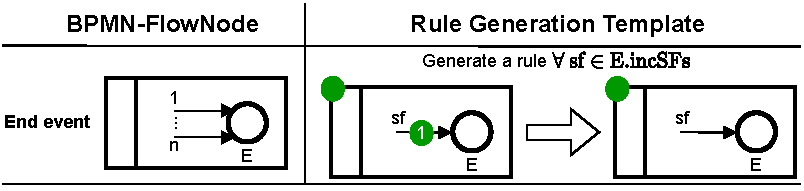
\includegraphics[width=.8\textwidth]{images/end_template.pdf}
    \caption{Rule generation template for end events}
    \label{fig:endTemplate}
\end{figure}
    
% End Event
The generated end event rules delete tokens one by one for each incoming sequence flow.
However, they do not terminate processes.
% General termination rule
Process termination is implemented with a generic rule---independent of the input BPMN model---which is applicable to all process snapshots.
The termination rule in \autoref{fig:terminationRule} is automatically generated once during the HOT.
The rule changes the state of the process snapshot from running to terminated if it has neither tokens nor subprocesses.

\begin{figure}[ht]
    \centering
    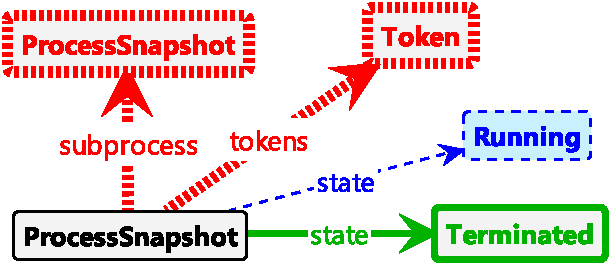
\includegraphics[width=.6\textwidth]{images/Terminate.pdf}
    \caption{Termination rule in Groove}
    \label{fig:terminationRule}
\end{figure}

The Groove syntax is the following.
The thin black elements in \autoref{fig:terminationRule} need to be present and will be preserved during transformation, while the dashed blue elements need to be present but will be removed.
Furthermore, the fat green elements will be created and the dashed fat red elements represent the NACs, whose presence prevent the rule from being applied.

\subsection{Activities \& Subprocesses}

% Normal activities
\autoref{fig:activityTemplates} depicts the rule generation templates for activities and subprocesses (see \autoref{fig:bpmnelementsOverview}).
Activity execution is divided into two steps implemented in parts \textbf{(a)} and \textbf{(b)} in the rule generation template \textbf{(1)}.
Part \textbf{(a)} generates one rule for each incoming sequence flow to start the activity.
An activity can be started using a token positioned at any of its incoming sequence flows.
This part generates the sample rule on the left of \autoref{fig:gtRuleConcrete}.
Having multiple incoming or outgoing sequence flows for a flow node is considered bad practice since the implicitly encoded gateways should be explicit to avoid confusion.
Our formalization still supports those models not to force modelers to rewrite them, but we recommend using static analyzers to avoid such models \cite{camundaservicesgmbhBpmnlint2023}.

Part \textbf{(b)} generates one rule that terminates the activity.
It deletes a token at the activity and adds one at each outgoing sequence flow.
This implicitly encodes a parallel gateway (see \autoref{fig:gatewayTemplates}) but should be avoided, as described earlier. 

% Could be split up into two figures
\begin{figure}[ht]
    \centering
    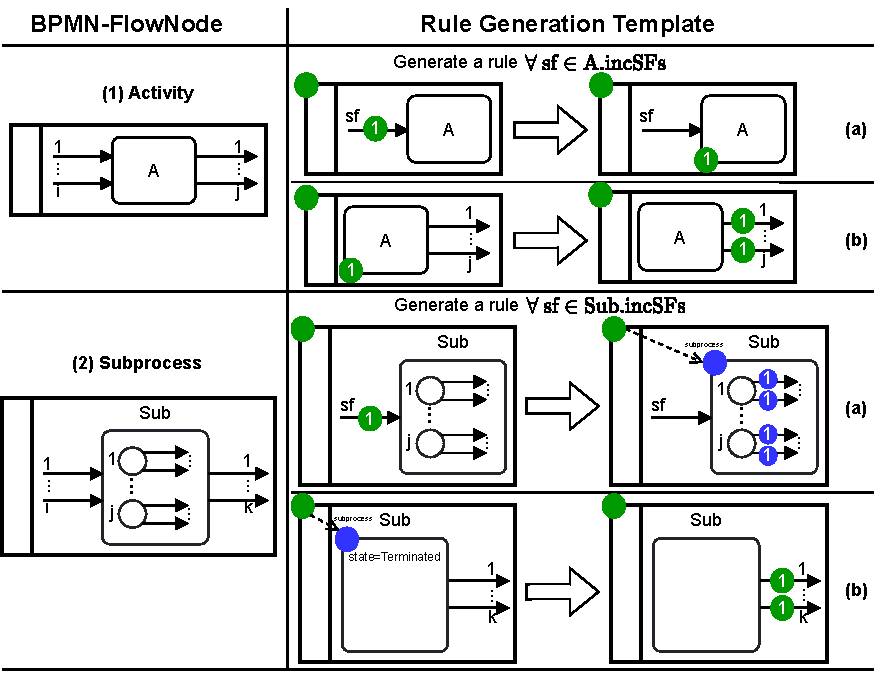
\includegraphics[width=1\textwidth]{images/activities_template.pdf}
    \caption{Rule generation template for activities and subprocesses}
    \label{fig:activityTemplates}
\end{figure}

% Subprocesses/Call activities
Subprocess execution is like activity execution.
Part \textbf{(a)} of the template generates one rule for each incoming sequence flow.
The rule deletes an incoming token and adds a process snapshot representing a subprocess. 
The created process snapshot is represented with a colored circle on the top left corner of the subprocess with a token at each outgoing sequence flow of its start events (similar to start graph generation).
There is a \textit{subprocess} link between the process snapshots to depict the \textsf{subprocesses} relation in \autoref{fig:bpmnExecutionMetamodel}.
If the subprocess has no start events, a token will be added to every activity and gateway with no incoming sequence flows.

Part \textbf{(b)} of the template generates one rule to delete a terminated process snapshot and adds tokens at each outgoing sequence flow.
Subprocesses are terminated by the termination rule (see section \ref{subsec:instAndTermination}).


% Send/Receive tasks (mentioned/shown with message events later)
\subsection{Gateways}
\autoref{fig:gatewayTemplates} depicts the rule generation templates for parallel and exclusive gateways (see \autoref{fig:bpmnelementsOverview}).
A parallel gateway can synchronize and fork the control flow simultaneously.
Thus, one rule is generated that deletes one token from each incoming sequence flow and adds one to each outgoing sequence flow.

\begin{figure}[ht]
    \centering
    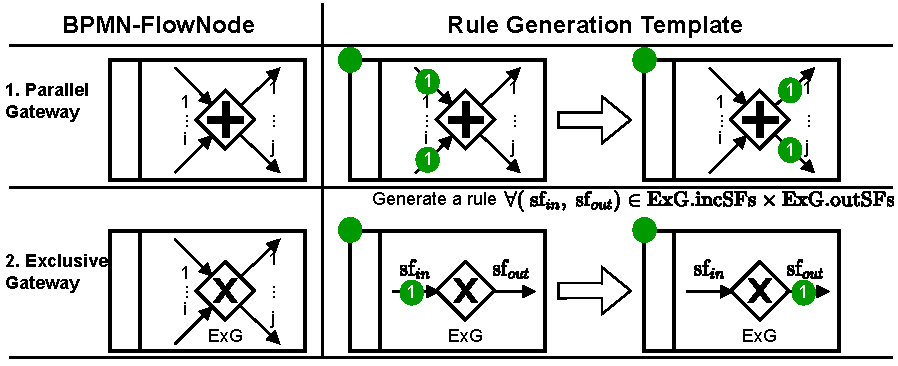
\includegraphics[width=1\textwidth]{images/gateways_template.pdf}
    \caption{Rule generation template for gateways}
    \label{fig:gatewayTemplates}
\end{figure}

Exclusive Gateways are triggered by exactly one incoming sequence flow, and exactly one outgoing sequence flow will be triggered as a result.
In practice, boolean conditions using data attached to the process are attached to exclusive gateways that decide which outgoing sequence flow to follow.
We do not model data flow in our formalization and instead allow each outgoing sequence flow to be explored. 
Thus, one rule must be generated for every combination of incoming and outgoing sequence flows.
However, the resulting rule is simple since it only deletes a token from an incoming sequence flow and adds one to an outgoing sequence flow.

\subsection{Message Events}
% General description
Message events are events directed at a single recipient.
Thus, they are unicast compared to broadcast signal events discussed later in \autoref{subsec:signalEvents}.
% Rule template description
% MITE
\autoref{fig:messageThrowEventTemplates} depicts the rule generation templates for \textit{message intermediate throw events} (\textsf{MITE} in \autoref{fig:bpmnelementsOverview}).
% MITE with MICE
Rule generation template \textbf{(1)} describes how MITEs interact with \textit{message intermediate catch events} (MICEs).
A MITE deletes an incoming token and adds one at each outgoing sequence flow.
In addition, it sends one message to each process by adding it to the incoming messages of the process.
However, sending each message is optional, meaning that if a process is not ready to consume a message immediately, the message is not added.
A process can consume a message if its MICE has at least one token at an incoming sequence flow (see rule template (1) in \autoref{fig:messageThrowEventTemplates}).
We implement optional message sending using nested rules with quantification.
Concretely, we use an optional existential quantifier \cite{rensinkNestedQuantificationGraph2006} (see dotted rectangle labeled \textsf{Optional} in \autoref{fig:messageThrowEventTemplates}) to send a message only if the receiving process is ready to consume it.

% MITE with MSE
Rule generation template \textbf{(2)} describes how MITEs interact with Message Start Events (MSEs).
For each MSE, a new process snapshot is created with tokens located at its outgoing sequence flows.
We split the interaction of MITEs with MICEs and MSEs into two rule templates for better understanding.
However, a MITE might interact with MICEs and MSEs simultaneously.
Thus, our HOT implements a merge of both templates. 
\textit{Message end events} (\textsf{MEE}) behave similarly to MITEs but only delete incoming tokens and do not add outgoing tokens.

\begin{figure}[ht]
    \centering
    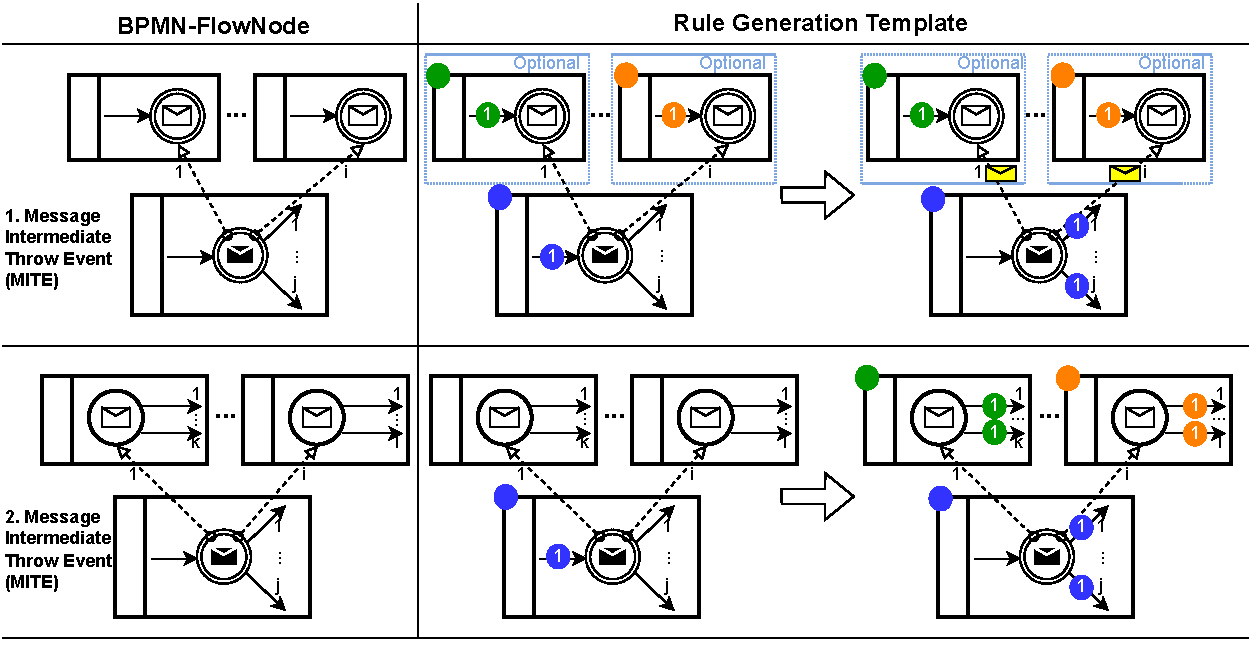
\includegraphics[width=1\textwidth]{images/mite_template.pdf}
    \caption{Rule generation templates for MITEs interacting with MICEs \textbf{(1)} and MSEs \textbf{(2)}}
    \label{fig:messageThrowEventTemplates}
\end{figure}

% MICE
The rule generation template in \autoref{fig:messageCatchEventTemplates} shows the behavior of \textit{message intermediate catch events} (\textsf{MICE} in \autoref{fig:bpmnelementsOverview}).
To trigger a MICE, only one message at an incoming \textit{message flow} is needed.
Thus, one rule is generated for each incoming \textit{message flow}.
The rule template shows that MICEs delete one message and one token, as well as add a token at each outgoing sequence flow.

\begin{figure}[ht]
    \centering
    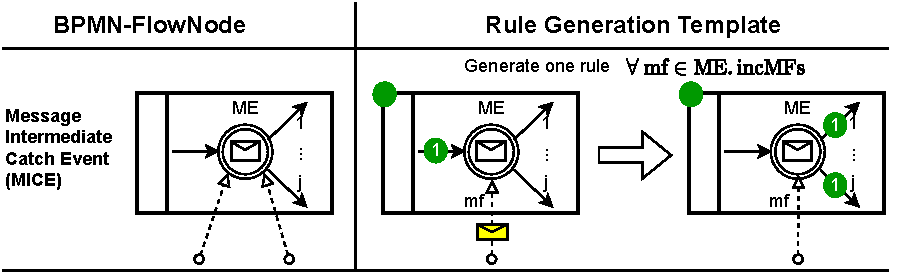
\includegraphics[width=0.8\textwidth]{images/mice_template.pdf}
    \caption{Rule generation templates for MICEs}
    \label{fig:messageCatchEventTemplates}
\end{figure}


\subsection{Link Events} \label{subsec:signalEvents}
% General description
Link events are similar to \enquote{Go To} statements since they move tokens from link throw events to link catch events in the same process level (cannot link to subprocesses).
They are meant to avoid long sequence flows and connect BPMN models spanning multiple pages but can also be used to create loops due to their \enquote{Go To} nature \cite{objectmanagementgroupBusinessProcessModel2013}.
\autoref{fig:linkEventTemplates} depicts the rule generation template for link throw events (LTEs), see \textsf{LTE} in \autoref{fig:bpmnelementsOverview}.
It shows how LTEs interact with link catch events (LCEs).

\begin{figure}[ht]
    \centering
    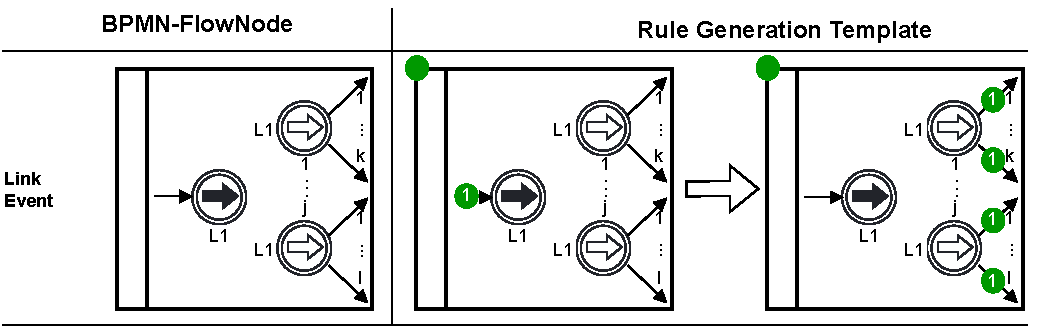
\includegraphics[width=1\textwidth]{images/linkEvent_template.pdf}
    \caption{Rule generation template for LTEs interacting with LCEs}
    \label{fig:linkEventTemplates}
\end{figure}

% Rule template description
Each rule deletes a token at that sequence flow and adds tokens to all outgoing sequence flows of matching LTEs.
An LTE matches an LCE if they have the same name.
In addition, they match despite different names if they have the same linked event definition (see \cite{objectmanagementgroupBusinessProcessModel2013}).
Our HOT automatically finds matching LTEs during transformation and then applies the rule template shown in \autoref{fig:linkEventTemplates}.

\subsection{Signal Events}
% General description
Each signal event references a named signal.
Signal throw events \textit{broadcast} to all signal catch events with the same signal.
Signal broadcasts have a global scope, i.e., they can communicate across process levels and pools \cite{objectmanagementgroupBusinessProcessModel2013}.

\autoref{fig:terminateEventTemplate} depicts the rule generation template for \textit{signal intermediate throw events} which interact with \textit{signal intermediate catch events} and \textit{signal start events} (\textsf{SITE}, \textsf{SICE}, and \textsf{SSE} in \autoref{fig:bpmnelementsOverview}).
\textit{Signal end events} (\textsf{SEE}) behave similarly to SITEs but only consume incoming tokens and do not add outgoing tokens.

\begin{figure}[ht]
    \centering
    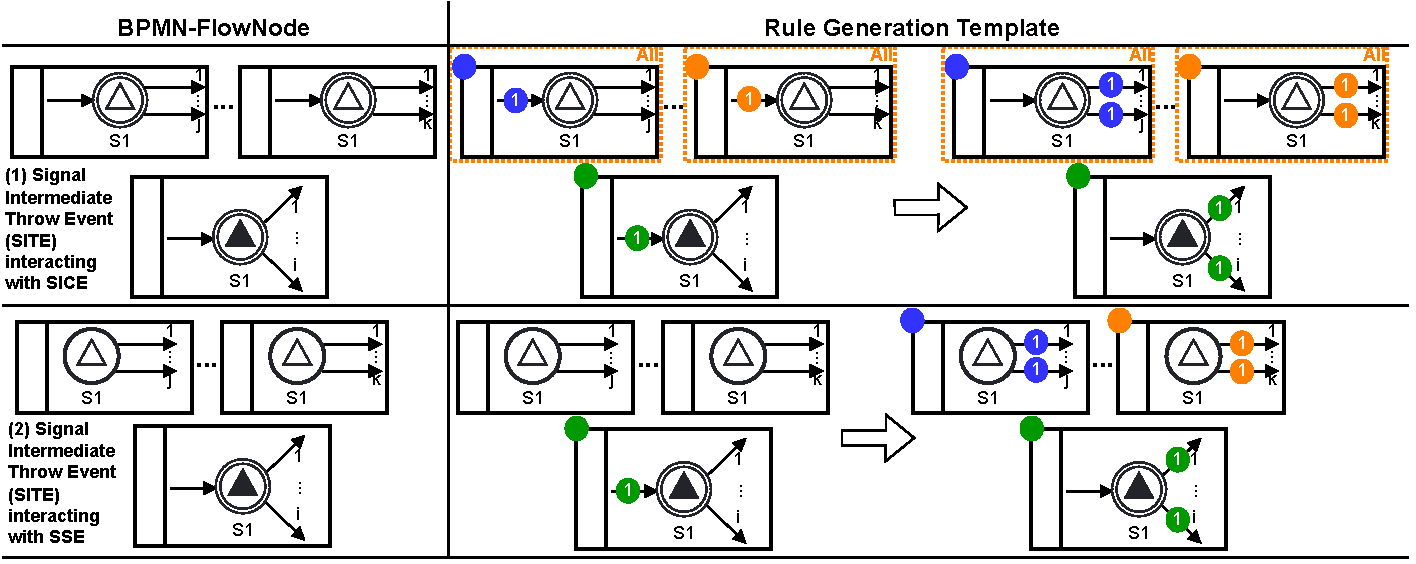
\includegraphics[width=1\textwidth]{images/signal_rule_template.pdf}
    \caption{Rule generation templates for SITEs interacting with SICE \textbf{(1)} and SSE \textbf{(2)}}
    \label{fig:signalEventTemplates}
\end{figure}

% Rule template description
Rule generation template \textbf{(1)} describes how SITEs interact with SICE.
Like other intermediate events, the incoming token is consumed while one token is added for each outgoing sequence flow.
Due to its broadcast semantics, a SITE interacts with all matching SICEs with an incoming token.
A SITE and SICE match if they have the same signal name.
In our templates, we assume that the signal name is the SITE/SICE name.
For each matching SICE, a universally quantified nested rule consumes the incoming token and adds a token for each outgoing sequence flow.
We use a universal quantifier (\textsf{All} in \autoref{fig:signalEventTemplates}) since one process snapshot might have multiple tokens waiting before a SICE.
Then, a SITE should trigger this SICE multiple times.

Rule generation template \textbf{(2)} describes how SITEs interact with SSEs.
Analogous to MITEs and MSEs, new process snapshots with tokens at the outgoing sequence flows of the SSEs are added for each matching SSE.
Each matching SSE is only triggered once, meaning we do not need any quantified nested rules.
% Merge of both templates
We split the interaction of SITEs with SICEs and SSEs into two rule templates for better understanding.
However, a SITE might interact with SICEs and SSEs simultaneously.
Thus, our HOT implements a merge of both templates.

\subsection{Terminate Events}
% General description
A terminate end event (TEE) abnormally terminates the running process \cite{objectmanagementgroupBusinessProcessModel2013}, meaning the process changes its state to terminated, and all its tokens are consumed.
\autoref{fig:terminateEventTemplate} depicts the rule generation template for \textit{terminate end events} (\textsf{TEE} in \autoref{fig:bpmnelementsOverview}).

\begin{figure}[ht]
    \centering
    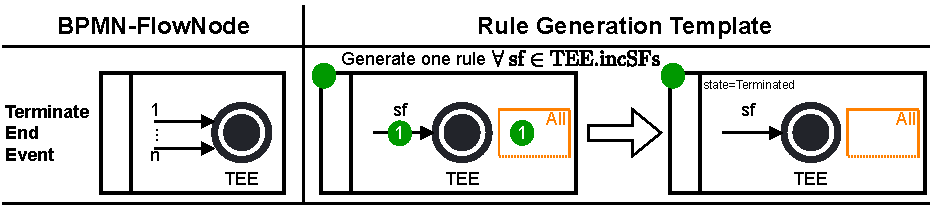
\includegraphics[width=0.8\textwidth]{images/terminate_end_event_template.pdf}
    \caption{Rule generation template for terminate end events}
    \label{fig:terminateEventTemplate}
\end{figure}

% Rule template description
One rule is generated for each incoming sequence flow of a TEE.
The rule consumes the incoming token, similar to the rules for end events, but also changes the process snapshot state to \textsf{Terminated}.
In addition, the rule deletes all other tokens of the process snapshot using a universally quantified nested rule (see dotted rectangle labeled \textbf{All} in \autoref{fig:terminateEventTemplate}).
Terminating a process must also terminate its subprocesses, which is not shown in the rule template in \autoref{fig:terminateEventTemplate} for brevity; it is described in our wiki \cite{timkrauterLMCS2024Artifacts2023}.

\section{Model checking BPMN} \label{sec:modelChecking}

Model checking ---and verification in general--- of BPMN models is necessary to ensure the correctness and reliability of business processes, which ultimately leads to increased efficiency, reduced costs, and user satisfaction.
Using our formalization approach, BPMN models may be verified against behavioral properties ---both general and user-defined--- by utilizing the generated GT system (see \autoref{fig:approach}).
These behavioral properties are defined using temporal logic, such as Computation Tree Logic (CTL) and Linear Temporal Logic (LTL) \cite{baierPrinciplesModelChecking2008}.
% Using our approach, model checking a BPMN model is possible using the generated GT system and behavioral properties based on atomic propositions (see \autoref{fig:approach}).
% Behavioral properties are defined using a temporal logic, such as CTL and LTL.
As mentioned in section bla, modelers may use our approach to specify user-defined properties consisting of atomic propositions and logical operators from CTL.
The atomic propositions are transformed to graph conditions by the HOT.
A graph condition is a GT rule which does not delete or add elements.
A proposition holds in a given state if a match of the graph condition exists in the graph representing the state \cite{kastenbergModelCheckingDynamic2006}.

We differentiate between two types of behavioral properties: \textit{general BPMN properties} defined for all BPMN models and \textit{custom properties} tailored towards a particular BPMN model.
We do not consider structural properties (like conformance to the syntax of BPMN) since they can be checked using a standard modeling tool without implementing execution semantics.
We will now give an example of two predefined general BPMN properties and show how they can be checked using our approach.
Then, we describe how custom properties can be defined and checked.

\subsection{General BPMN properties}
\textit{Safeness} and \textit{Soundness} properties are defined for BPMN in \cite{corradiniClassificationBPMNCollaborations2018}.
A BPMN model is \textit{safe} if, during its execution, at most one token occurs along the same sequence flow \cite{corradiniClassificationBPMNCollaborations2018}.
Soundness is further decomposed into (i) \textit{Option to complete}: any running process instance must eventually complete, (ii) \textit{Proper completion}: after completion, each token of the process instance must be consumed by a different end event, as well as (iii) \textit{No dead activities}: each activity can be executed in at least one process instance \cite{corradiniClassificationBPMNCollaborations2018}.
Process completion is synonymous with process termination.
In the following, we will describe how to implement the \textit{Safeness} and \textit{Option to complete} properties.

% Safeness
We specify \textit{Safeness} as the CTL property defined in \eqref{eq:safeness}.
% TODO: describe CTL \cite{baierPrinciplesModelChecking2008}
The atomic proposition \textsf{Unsafe} is true if two tokens of one process snapshot point to the same sequence flow.
It is shown in \autoref{fig:unsafe} using abstract Groove syntax.

\begin{figure}[ht]
    \centering
    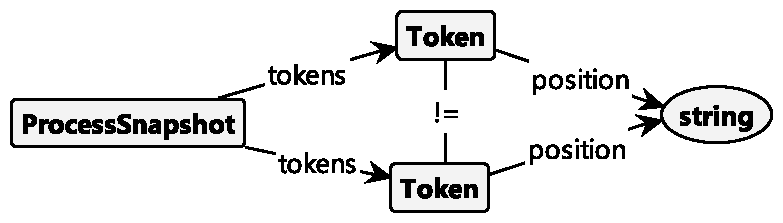
\includegraphics[width=0.8\textwidth]{images/Unsafe.pdf}
    \caption{The atomic proposition \textit{Unsafe} as a Groove graph condition.}
    \label{fig:unsafe}
\end{figure}

\begin{figure}[ht]
    \centering
    
\includegraphics[width=0.5\textwidth]{images/AllTerminated.pdf}
    \caption{The atomic proposition \textit{AllTerminated} as a Groove graph condition.}
    \label{fig:allTerminated}
\end{figure}

% Option to complete
\textit{Option to complete} is specified using the CTL property defined in \eqref{eq:optionToComplete}.
The atomic proposition \textsf{AllTerminated} is true if there exists no process snapshot in the state \textsf{Running}, i.e., all process snapshots are \textsf{Terminated}.
It is shown in \autoref{fig:allTerminated} using abstract Groove syntax.

\noindent\begin{minipage}{.5\linewidth}
\begin{equation} \label{eq:safeness}
  AG(\neg \,\text{Unsafe})
\end{equation}
\end{minipage}%
\begin{minipage}{.5\linewidth}
\begin{equation} \label{eq:optionToComplete}
  AF(\text{AllTerminated}) 
\end{equation}
\end{minipage}
\vskip.3\baselineskip

Checking the properties \textit{Safeness}, \textit{Option to Complete}, and \textit{No Dead Activities} is implemented in our tool \cite{timkrauterLMCS2024Artifacts2023}.
The property \textit{Proper Completion} is not yet implemented, but all the information needed can be found in the GT systems state space.

\subsection{Custom properties} \label{subsec:customProperties}
% Defining atomic propositions in BPMN is a novelty.
% To make model checking user-friendly, we envision modelers defining atomic propositions based on the extended BPMN syntax, i.e., the concrete syntax introduced in \autoref{fig:bpmnExecutionMetamodel}.
% Therefore, a modeler adds process snapshots and tokens to a BPMN model to define an atomic proposition, which we can automatically convert to a GT rule representing an atomic proposition.
% GT rules representing atomic propositions are not allowed to delete or add elements and are called graph conditions in Groove.
% Furthermore, a modeler can define that a token should not exist at a given position, which leads to NACs in the graph condition. 


To make model checking user-friendly, we enable modelers to define atomic propositions using the concrete syntax of the extended BPMN execution metamodel introduced in \autoref{fig:bpmnExecutionMetamodel} (see \autoref{fig:shippedTwiceProposition}).
An atomic proposition is defined as a process snapshot, together with a token distribution (see \autoref{fig:shippedTwiceAbstractAndGroove}A), which we can automatically convert to a graph condition in Groove (see \autoref{fig:shippedTwiceAbstractAndGroove}B).
Recall that graph conditions are GT rules that are run in check mode, i.e., the are not allowed to delete or add elements.
Atomic propositions may be connected by simple CTL-operators such as \textsf{G, F, $\to$} to create temporal formulae which should hold in the given BPMN model. 
Furthermore, modelers may forbid certain states in the BPMN model by specifying that a certain token distribution should not should not exist.
These situations would lead to Negative Application Conditions (NACs) in the graph conditions. 


For example, the token distribution shown in \autoref{fig:shippedTwiceProposition} defines a process snapshot with two tokens at activity \textit{Ship goods}.
A modeler could use this atomic proposition to check if the activity \textit{Ship goods} is executed twice by creating an appropriate LTL/CTL property.
Shipping goods twice but only receiving one payment during an order-handling process would be a critical error for a business.
The order handling process in \autoref{fig:shippedTwiceProposition} is taken from \cite{ruckerPracticalProcessAutomation2021} but changed to contain a modeling error.
The modeling error leads to potentially shipping goods twice if the process is not corrected before deployment.

\begin{figure}[ht]
    \centering
    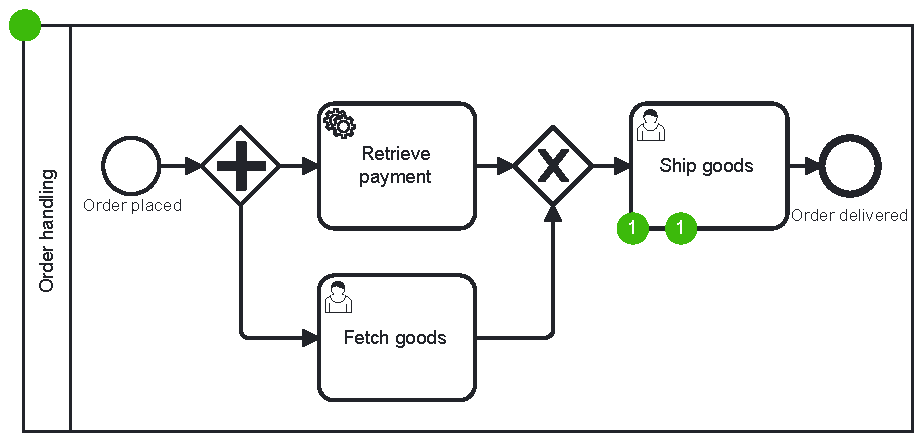
\includegraphics[width=0.65\textwidth]{images/shippedTwiceProposition.pdf}
    \caption{Atomic proposition defining shipping goods twice.}
    \label{fig:shippedTwiceProposition}
\end{figure}

\begin{figure}[ht]
    \centering
    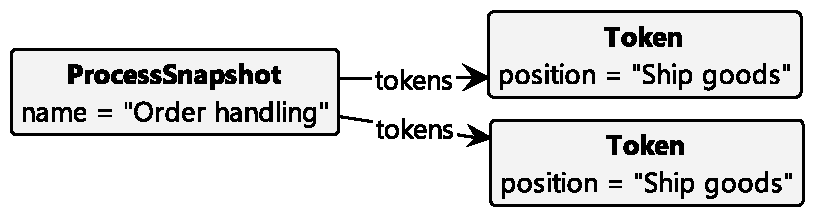
\includegraphics[width=1\textwidth]{images/twice.pdf}
    \caption{Abstract syntax \textbf{(a)} and graph condition in Groove \textbf{(b)} for \autoref{fig:shippedTwiceProposition}}
    \label{fig:shippedTwiceAbstractAndGroove}
\end{figure}

Another proposition for the same erroneous process is shown in \autoref{fig:shippingAfterPayment}.
The proposition defines that when the activity \textit{Ship goods} runs (has a token), the activity \textit{Retrieve payment} should not run (has no token) in the same process instance.
\enquote{Has no token} is depicted by crossing out the token symbol and represents an extension of our concrete syntax introduced for defining propositions.
This proposition can be used to define a property to check if shipping ever occurs while retrieving payments has not been completed yet.
The GT system for the order handling process containing both propositions can be found in \cite{timkrauterLMCS2024Artifacts2023}.

\begin{figure}[ht]
    \centering
    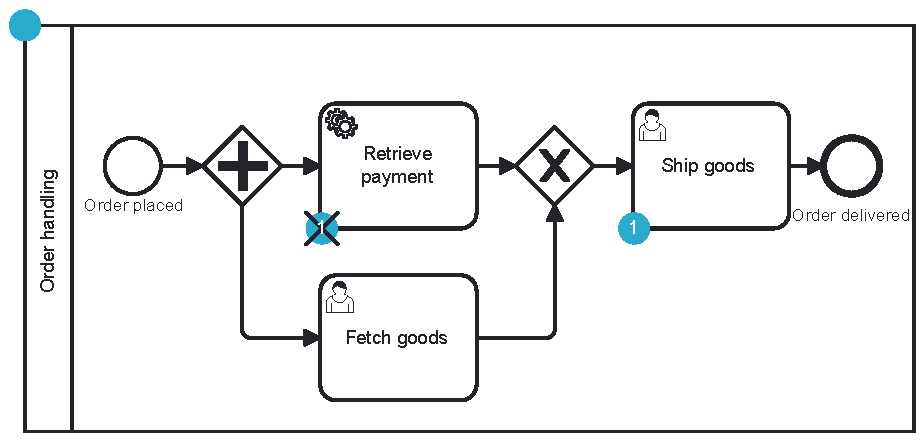
\includegraphics[width=0.65\textwidth]{images/shippingAfterPayment.pdf}
    \caption{Atomic proposition defining shipping after retrieving payment.}
    \label{fig:shippingAfterPayment}
\end{figure}

% Using a proposition editor based on our concrete syntax, a modeler can work with BPMN, which is well-known to him.
% He does not need to define his propositions in the GT semantics used for execution since each proposition is automatically transformed as described earlier.
% To summarize, many propositions can defined using this simple method.

Using an atomic proposition-editor based on the BPMN concrete syntax, modelers would not need to have extensive knowledge about the GT-based execution semantics. 
% However, the expressibility is not the same as in the GT semantics.
% For example, one can use nested rules with quantification in graph conditions in Groove.
% Thus, when defining a proposition editor, there is a clear tradeoff between \textit{simplicity} and \textit{expressibility}.
% Currently, we favor simplicity in our tool and recommend defining propositions in GT semantics if more powerful constructs are needed.
% In addition, expressibility varies and is achieved differently in GT tools, and we try to stay as independent as possible from specific GT tools.
Although the expressiveness is not as powerful as in the GT-based execution semantics in Groove---e.g., one can use nested rules with quantification in graph conditions---we favor \textit{simplicity} over \textit{expressiveness}.
In addition, we attempt to stay as independent as possible from the framework and tools used for the execution semantics (see the right module of \autoref{fig:approach}). %, and specific GT tools expressibility varies in this bla.

Finally, the modeler must still know the temporal logic, such as LTL and CTL, to express his properties.
To combat this problem, we added temporal logic templates to our tool to generate commonly occurring propositions without knowledge about temporal logic.
This feature is discussed in detail in the implementation section.
In the future, a domain-specific property language for BPMN would further lessen the knowledge required from the modeler \cite{meyersProMoBoxFrameworkGenerating2014}.

\section{Implementation} \label{sec:impl}
In this section, we will present our tool, the BPMN Analyzer, which greatly improves the version published in \cite{krauterFormalizationAnalysisBPMN2023}.
In addition, we will describe initial performance experiments of the tool.

\subsection{BPMN Analyzer}

Our approach is implemented as a web-based tool called \textit{BPMN Analyzer}, which is open-source, publicly available, and does not require any installation \cite{timkrauterLMCS2024Artifacts2023, krauterFormalizationAnalysisBPMN2023}.
\autoref{fig:implScreenshot} depicts a screenshot of the BPMN Analyzer.
We use the order handling process from \cite{ruckerPracticalProcessAutomation2021} as an example.
It is the same BPMN model as in \autoref{fig:shippedTwiceProposition} and \autoref{fig:shippingAfterPayment} but without modeling errors.

The modeler can create or upload a BPMN model, which can then be verified using either general BPMN properties or custom properties formulated in CTL.
BPMN Analyzer generates a GT system for the supplied BPMN model and runs model checking against the specified properties in Groove \cite{kastenbergModelCheckingDynamic2006}. 
To evaluate the correctness of our HOT, we have created a comprehensive test suite \cite{timkrauterLMCS2024Artifacts2023}.
It verifies that rules are generated as defined by the rule generation templates in the previous section for each BPMN element.

\begin{figure}[ht]
    \centering
    \frame{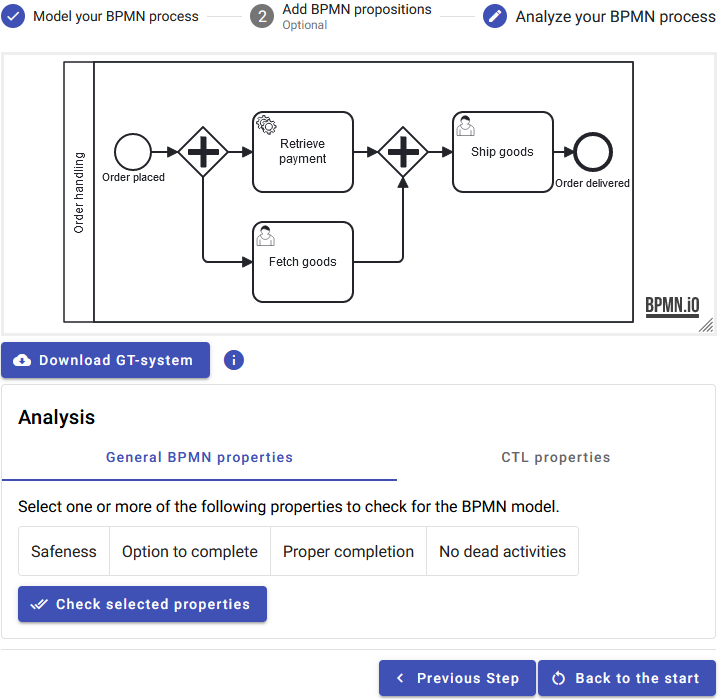
\includegraphics[width=.9\textwidth]{images/impl_step3.png}}
    % 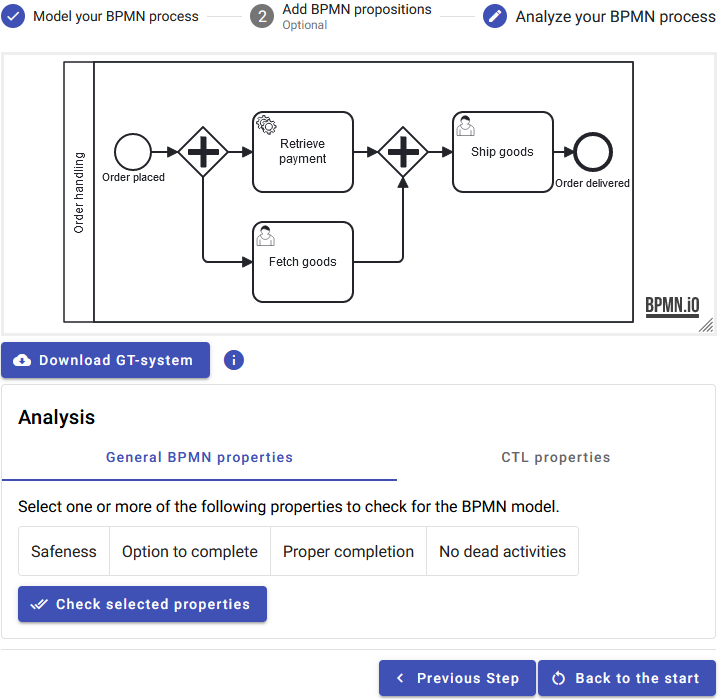
\includegraphics[width=1\textwidth]{images/impl_step3.png}
    \caption{Screenshot of the \textit{analysis step} in the BPMN Analyzer tool}
    \label{fig:implScreenshot}
\end{figure}

% We significantly improved the BPMN Analyzer tool for this extended version.
% First, we improved the usability of the tool.
% We restructured the user interface, previously contained on one page, into three distinct steps while adding new features.
% The user is transparently guided through these three steps by the application flow.

The BPMN Analyzer interface is structured into three distinct sections where the user is transparently guided through the modeling and analysis processes by the application flow.

\begin{enumerate}
  \item The \textbf{Modeling} section lets users upload or define the BPMN model.
  We utilize a properties panel in the modeling step such that IDs of BPMN elements can be viewed and edited directly in the model editor.
  This allows for better traceability between BPMN elements and generated GT rules when a user chooses to inspect the generated GT system.
  \item The \textbf{Custom Propositions} section contains the atomic proposition editor.
  In this section, users may create atomic propositions, which may be used as ingredients using the custom properties builder.
  Users who are only interested in general BPMN properties may skip this step.
  Atomic propositions are created using the concrete syntax detailed in \autoref{subsec:customProperties}, which is implemented as a custom diagram editor.
  As mentioned, to create a proposition, users attach tokens and process snapshots to the BPMN model created in the modeling section.
  %We implemented a custom diagram editor for this step to achieve the best possible usability.
  \item In the \textbf{Analysis} section, users may check the general BPMN properties and build custom properties using the atomic propositions. 
  The properties builder utilizes a textual CTL-syntax to specify custom properties using the atomic propositions from the previous section.
  %Second, 
  The CTL properties builder comes with CTL templates to facilitate commonly occurring CTL properties.
  These templates allow currently for checking whether a state (described by an atomic proposition) can be reached or not.
  Thus, simple safety and liveness properties can be checked using these templates.
  Users who download the generated GT system may inspect and edit the graph conditions generated from the atomic propositions; they may also specify more properties in their favorite temporal logic and check them using Groove.
  Model-checking experts in an organization can define more templates in the future and share them for reuse. 

\end{enumerate}


% we added CTL templates to the analysis of the step such that a modeler can generate commonly occurring CTL propositions.
% He selects a template and a proposition to generate a CTL property.
% So far, we have added two templates for checking if a state (described by a proposition) can be reached or is never reached.
% Thus, simple safety and liveness properties can be checked using these templates.
% Model-checking experts in an organization can define more templates in the future and share them for reuse. 


\subsection{Ruseable libraries}
In addition to the BPMN Analyzer, we published multiple parts of our application as libraries such that they can be reused seamlessly by other researchers and practitioners.
The BPMN metamodel extension needed to define custom propositions is published as an npm module (\textit{token-bpmn-moddle}) \cite{timkrauterLMCS2024Artifacts2023}.
Npm is the default package manager for the JavaScript programming language.
In addition, the BPMN token editor to define atomic propositions is also published as an npm module (\textit{token-bpmn}) \cite{timkrauterLMCS2024Artifacts2023}.
Furthermore, we published our \textit{graph-rule-generation} library to generate Groove GT systems to the Maven central repository \cite{timkrauterLMCS2024Artifacts2023}.
The Maven central repository is the standard repository for developing JVM-based applications.
We explain each library in detail in the following sections.

\subsubsection{BPMN metamodel extension}
% Same concrete syntax but slightly different to fit the UI/proposition needs.
Our implementation \textit{token-bpmn-moddle} \cite{timkrauterLMCS2024Artifacts2023} extends \textit{bpmn-moddle} \cite{camundaservicesgmbhBpmnmoddle2023}, which implements the BPMN specification.
Our extension adds the \textsf{Token} and \textsf{ProcessSnapshot} types from the BPMN execution metamodel shown in \autoref{fig:bpmnExecutionMetamodel} to the BPMN metamodel.
\autoref{lst:extension} shows an example BPMN XML snippet, where a token and process snapshot was added.

\lstinputlisting [label=lst:extension, language=XML, numbers=left,
    stepnumber=1, caption=BPMN XML snippet showing an example of our BPMN metamodel extension]{./listings/extension.xml}

The library allows one to create token and process snapshot instances and stores them in the BPMN extension elements (lines 2-5 in the XML example in \autoref{lst:extension}).
This is the recommended way to extend the BPMN metamodel \cite{objectmanagementgroupBusinessProcessModel2013}.
We use an association (lines 7-8 in \autoref{lst:extension}) to define the element at which the token is located, i.e., the token's \textsf{elementID} (see BPMN execution metamodel in \autoref{fig:bpmnExecutionMetamodel}).
This XML model is consumed by our HOT to generate atomic propositions for Groove (see \autoref{fig:approach}).
However, following sound model-driven principles and creating an extended metamodel, the XML model could also be used in other applications or for model checking with different tools.

\subsubsection{BPMN token editor}
The BPMN token editor implements the concrete syntax for tokens and process snapshots described in \autoref{fig:bpmnExecutionMetamodel}.
Using our token editor, a user does not need to write XML since the complexity of extending the BPMN metamodel described in the previous chapter is hidden in the editor.

\autoref{fig:tokenEditor} shows the token editor embedded in the second step of the BPMN Analyzer.
We simplify the user interface so users can only edit tokens and process snapshots, and not the underlying BPMN model.
Process snapshots are automatically assigned distinct colors, and tokens held by a process snapshot have the same color (see concrete syntax in \autoref{fig:bpmnExecutionMetamodel}).
Tokens can be assigned to process snapshots, which changes the token's color to match the snapshot.

\begin{figure}[ht]
    \centering
    \frame{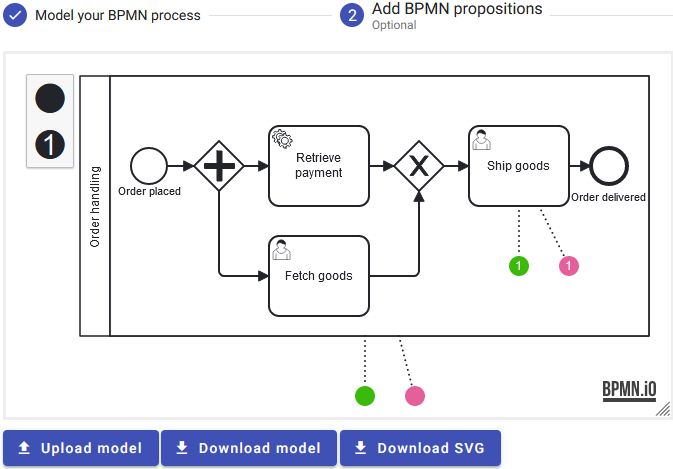
\includegraphics[width=0.9\textwidth]{images/impl_step2.png}}
    \caption{Screenshot of the BPMN token editor used in the BPMN Analyzer tool}
    \label{fig:tokenEditor}
\end{figure}

Our implementation is based on \textit{bpmn-js} \cite{camundaservicesgmbhBpmnjs2023}, which provides a BPMN rendering toolkit and uses the \textit{token-bpmn-moddle} library described in the previous section to save and load our models.
Since both implementations are published as libraries, they can be easily reused in other applications.

\subsubsection{Graph rule generation}
The graph-rule-generation library offers different classes to generate graphs, GT rules, or entire GT systems, following the \textit{builder pattern} \cite{gammaDesignPatternsElements1995}.
\autoref{lst:grooveRuleBuilder} shows an example code snippet to generate a GT rule using the GT rule builder implemented for Groove.

\lstinputlisting [label=lst:grooveRuleBuilder, language=Java, numbers=left,
    stepnumber=1, caption=Code snippet to generate a GT rule using the Groove GT rule builder]{./listings/gtRuleBuilderSnippet.txt}

Using the rule builder, one can construct a GT rule by defining which nodes and edges should be present (lines 6-8), deleted (lines 10-12), added (lines 14-16), or NACs (lines 18-20), see \autoref{lst:grooveRuleBuilder}.
\autoref{fig:grooveRuleBuilderRule} shows the resulting GT rule specified by \autoref{lst:grooveRuleBuilder} in Groove syntax.

\begin{figure}[ht]
    \centering
    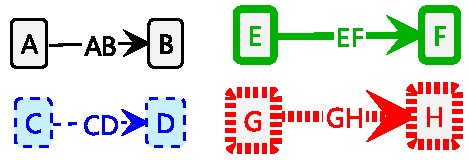
\includegraphics[width=0.5\textwidth]{images/rule.pdf}
    \caption{Groove GT rule generated by the code snippet in \autoref{lst:grooveRuleBuilder}}
    \label{fig:grooveRuleBuilderRule}
\end{figure}

Similarly to the groove rule builder in \autoref{lst:grooveRuleBuilder}, we also provide a builder for constructing graphs to create start graphs of GT systems \cite{timkrauterLMCS2024Artifacts2023}.
Finally, the library provides a builder for GT systems using the graph and GT rule builders.
The Groove UI and the Groove command-line tools can then consume the generated GT systems.

\subsection{Experiments}

Model checking is a useful technique but often falls short in practice due to insufficient performance.
Poor performance might have many reasons, most notably large models leading to state space explosion.
We experimented with ten different BPMN models from \cite{houhouFirstOrderLogicVerification2022} to assess the performance of our implementation.
We picked the models at random, but we disregarded some similar models.
The models include realistic business process models (e.g., 001, 002, and 020) \cite{houhouFirstOrderLogicVerification2022}.

To calculate the average runtime, we used the hyperfine benchmarking tool \cite{peterHyperfine2023} (version 1.18.0), which ran the HOT/state space exploration for each BPMN model ten times.
The experiment was run on Windows 11 (AMD Ryzen 7700X processor, 32 GB RAM) using Groove version 6.1.0 \cite{timkrauterLMCS2024Artifacts2023}.
Compared to \cite{krauterFormalizationAnalysisBPMN2023}, we used the newest HOT implementation as well as the newest Groove and hyperfine versions.

First, we ran our HOT for the BPMN models.
The HOT takes approximately half a second to generate a GT system for each model.
Thus, the generation of the GT systems for these models is fast enough.

Second, we ran a full state exploration using the resulting ten GT systems, see \autoref{table:stateSpaceBenchmark}.
The exploration takes around one second for most of the models.
Only model \textit{020} needs nearly two seconds due to its larger state space.
Furthermore, up to one second is spent on startup, not model checking.
For example, Groove reports only 722 ms for state space exploration for model \textit{020}.

We conclude that our approach is sufficiently fast for models of average size.
In addition, there is still room for optimization, such as avoiding costly I/O to disk or parallelizing the HOT.
In the next section, we test the scalability of our approach.
However, a comprehensive benchmark, including a detailed comparison to other tools, is left for future work.

\begin{table}[ht]
\centering
\caption{Experimental results for a full state space exploration in Groove}

\begin{tabular}{| c | c | c || c | c | c |}
 \hline
 BPMN model & Processes & Nodes (gw.) & States & Transitions & Total time \\
 \hline\hline
 001 & 2 & 17(2) & 68 & 118 & $\sim$ 1.00 s \\
 \hline
 002 & 2 & 16(2) & 62 & 108 & $\sim$ 0.97 s \\
 \hline
 007 & 1 & 8(2) & 45 & 81 & $\sim$ 0.92 s \\
 \hline
 008 & 1 & 11(2) & 49 & 85 & $\sim$ 0.93 s \\
 \hline
 009 & 1 & 12(2) & 137 & 308 & $\sim$ 1.01 s \\
 \hline
 010 & 1 & 15(2) & 162 & 357 & $\sim$ 1.04 s \\
 \hline
 011 & 1 & 15(2) & 44 & 69 & $\sim$ 0.97 s \\
 \hline
 015 & 1 & 14(2) & 53 & 86 & $\sim$ 0.95 s \\
 \hline
 016 & 1 & 14(2) & 44 & 68 & $\sim$ 0.94 s \\
 \hline
 020 & 1 & 39(6) & 3060 & 8584 & $\sim$ 1.75 s \\
 \hline
\end{tabular}
\label{table:stateSpaceBenchmark}
\end{table}

\section{Scalability test} \label{sec:scalability}

In this section, we test the scalability of our approach by applying it to 300 heterogeneous BPMN models with increasing model sizes. 

\subsection{Setup}

We generated 300 BPMN models to test the scalability of our approach.
We used the following approach to include different BPMN elements in our models.
We generated the models incrementally, increasing the number of \textit{blocks} they contain.
Thus, model one contains one block, model two contains two blocks, and so forth until the last model contains 300 blocks.
During the generation, we alternate between the three different blocks shown in \autoref{fig:blocks}.

\begin{figure}[ht]
    \centering
    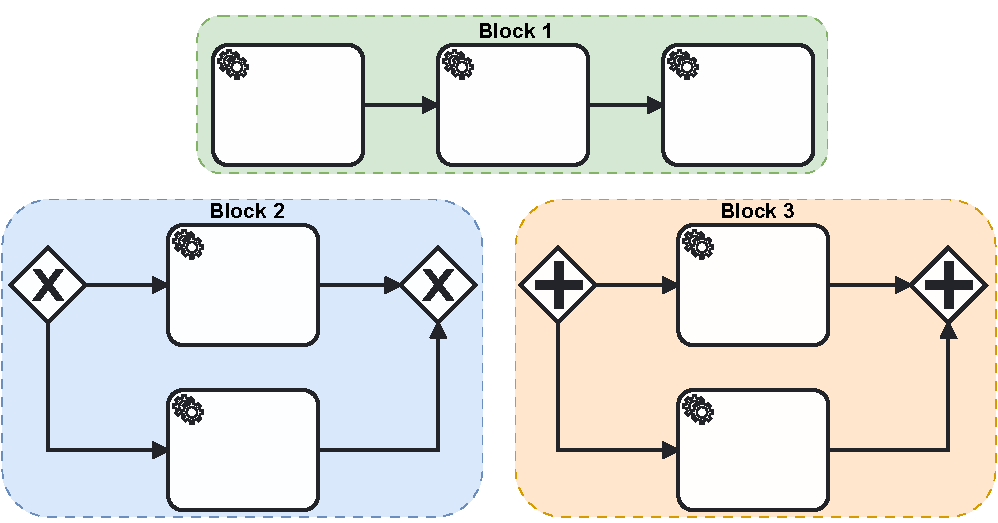
\includegraphics[width=0.8\textwidth]{images/blocks.pdf}
    \caption{The three different blocks used for BPMN model generation}
    \label{fig:blocks}
\end{figure}

For example, the BPMN model with three blocks is depicted in \autoref{fig:threeBlockModel}.
Blocks two and three are shown in a new line for better visualization.
However, the generated models are expanding horizontally in one line.
We then repeat adding one block at a time for each new model until we reach 300 models.

\begin{figure}[ht]
    \centering
    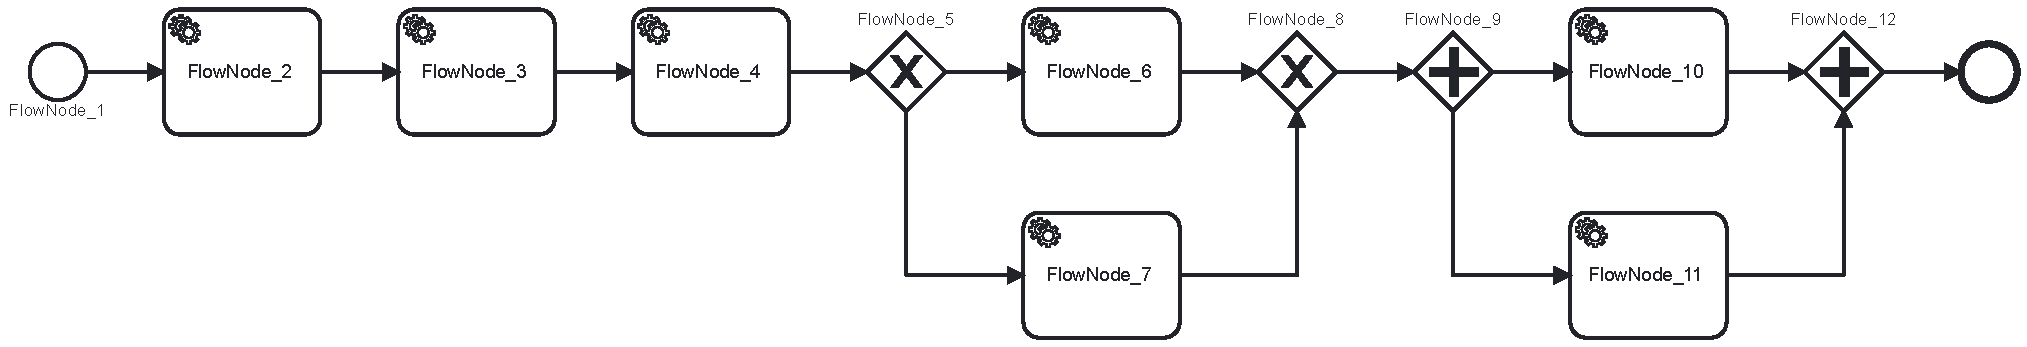
\includegraphics[width=1\textwidth]{images/003.pdf}
    \caption{A generated BPMN model with three blocks}
    \label{fig:threeBlockModel}
\end{figure}

\autoref{table:bpmnModelCharacteristics} states the characteristics of the generated BPMN models, such as the number of gateways, flow nodes, and sequence flows.
One can deduce from the table that adding fifty blocks adds around 400 BPMN elements to a model.
All models, including their characteristics and how to generate them, can be found in \cite{timkrauterLMCS2024Artifacts2023}.
Our BPMN model generation uses the camunda BPMN model API \cite{camundaservicesgmbhCamundaBPMNModel2023}.

BPMN models in practice tend to be much smaller since large models are usually divided into smaller submodels \cite{fahlandAnalysisDemandInstantaneous2011}, i.e., subprocesses, to ensure they are understandable by modelers.
Each of these subprocesses can then be analyzed independently.
From our experience and referring to other studies \cite{fahlandAnalysisDemandInstantaneous2011}, this best practice leads to models with less than 400 total elements (comparable to less than 50 blocks in \autoref{table:bpmnModelCharacteristics}).
We ran our scalability test for models with up to 300 blocks since we wanted enough data to see trends in the average runtime.
We did not go beyond 300 blocks since the whole test should still run in a reasonable time. 


\begin{table}[ht]
\centering
\caption{Characteristics of the generated BPMN models}
\begin{tabular}{| c | c | c | c || c |}
 \hline
 BPMN model / Blocks & Gateways & Flow nodes & Sequence flows & Total elements \\
 \hline\hline
 1 & 0 & 5 & 4 & 9 \\
 \hline
 50 & 66 & 185 & 217 & 402 \\
 \hline
 100 & 132 & 368 & 433 & 801 \\
 \hline
 150 & 200 & 552 & 651 & 1203 \\
 \hline
 200 & 266 & 735 & 867 & 1602 \\
 \hline
 250 & 332 & 918 & 1083 & 2001 \\
 \hline
 300 & 400 & 1102 & 1301 & 2403 \\
 \hline
\end{tabular}
\label{table:bpmnModelCharacteristics}
\end{table}

\subsection{Results}

% Description
\autoref{fig:hotScalability} depicts the results of benchmarking our HOT with the generated BPMN models.
It shows the average runtime of five runs for transforming each BPMN model into a GT system using our HOT.
We used the same machine and setup as discussed for our performance experiments in \autoref{sec:impl}.

\begin{figure}[ht]
    \centering
    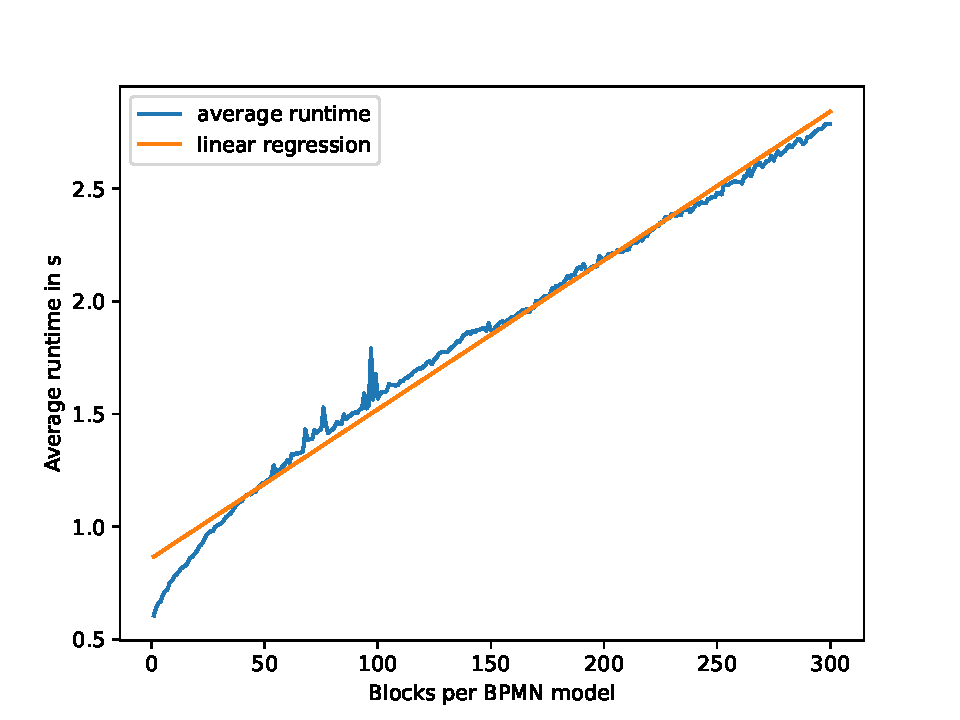
\includegraphics[width=0.8\textwidth]{images/HOT_scalability.pdf}
    \caption{Scalability testing result of the GT system generation}
    \label{fig:hotScalability}
\end{figure}

% Interpretation and takeaways
The average HOT runtimes data fits the linear regression shown in \autoref{fig:hotScalability} well.
This makes sense since the HOT algorithm has \textit{linear runtime complexity} because it iterates over all flow nodes of a BPMN model to generate GT rules.
We conclude that the HOT is fast enough (around one second or less) for models of reasonable size (50 blocks or less).

% Description
\autoref{fig:stateSpaceScalability} depicts the results of benchmarking the state space generation in Groove for the GT systems obtained by our HOT.
It shows the average runtime of five runs, calculated by hyperfine \cite{peterHyperfine2023}.

\begin{figure}[ht]
    \centering
    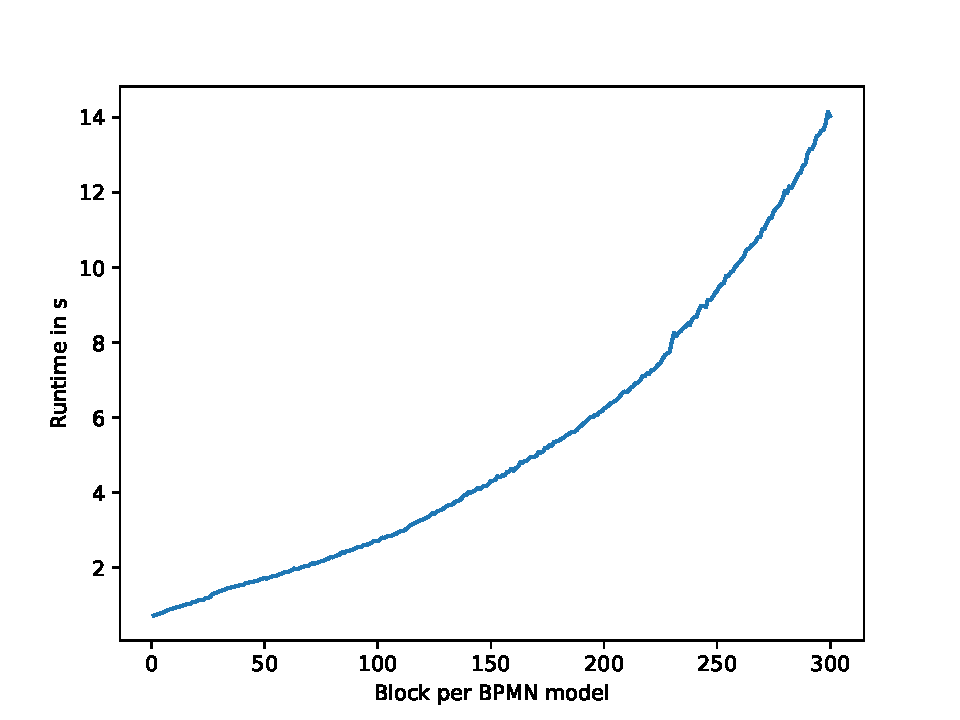
\includegraphics[width=0.8\textwidth]{images/StateSpaceGeneration_scalability.pdf}
    \caption{Scalability testing result of the state space generation in Groove}
    \label{fig:stateSpaceScalability}
\end{figure}

% Interpretation and takeaways
The increase in the runtime of the state space generation looks worse than linear.
However, models of reasonable size (50 blocks or less) are handled in less than two seconds.
To summarize, using our approach, we can conservatively estimate that these models can be checked (HOT followed by a full state space generation) in around three seconds or less.
In addition, a full-state space exploration is not always needed for model checking.

% Plenty of optimization potential
Plenty of optimization potentials exist, starting from the HOT and ending with the state space generation in Groove.
Currently, neither our HOT nor Groove are specifically optimized for performance with this use case in mind.
% HOT optimization
Regarding the HOT, multiple optimizations come to mind.
First, one can parallelize the generation of GT rules since each rule is independent.
Second, one can change the rule-generation templates to reduce the number of generated rules and the state space.
For example, two rules are currently generated to represent starting and finishing an activity (see \autoref{fig:activityTemplates}), which fits the description in the BPMN specification.
However, one could instead generate only one rule, which represents the whole execution of an activity.
Thus, one less rule is generated, and the intermediate state representing the activity executing is no longer part of the state space.
If there are many activities, especially when they are executed in parallel, this can lead to large reductions in the state space.
However, a less granular state space could prohibit checking certain properties.
A trade-off exists between staying close to the BPMN execution specification and overall runtime (HOT and state space generation).

% Groove optimization
Groove is a powerful tool with good out-of-the-box performance.
However, there is still optimization potential.
First, GT rules should not be written to and read from the disk to interact with Groove.
Each GT rule is saved to a new file, and the number of generated GT rules increases with the size of a BPMN model.
Integrating our HOT and Groove more tightly can eliminate these costly I/O operations since the generated rules can stay in the main memory.
This optimization is especially useful for our approach.
Second, \textit{partial order reduction} methods could greatly reduce the time and space required for model checking \cite{clarkeHandbookModelChecking2018}.
Third, Groove could use \textit{on-the-fly} model checking.
If a counterexample is found, there is no need to continue the state space generation \cite{clarkeHandbookModelChecking2018}.

\section{Related work} \label{sec:relatedWork}
% Petri nets formalisms
The most common formalizations of BPMN use Petri Nets.
For example, \cite{dijkmanSemanticsAnalysisBusiness2008} formalizes a subset of BPMN elements by defining a mapping to Petri Nets conceptually close to our HOT-based formalization.
% Difficulties with Petri net encodings
Encoding basic BPMN modeling elements into Petri Nets is generally straightforward, but for some advanced elements, it can be complicated to define \cite{hofstedeWorkflowPatternsExpressive2002}.
For example, representing \textit{termination end events} and \textit{interrupting boundary events}, which interrupt a running process, is usually unsupported because of the complexity of managing the non-local propagation of tokens in Petri Nets \cite{corradiniFormalApproachAnalysis2021}.
We solve these situations by using nested graph conditions, for example, to remove all tokens when reaching a \textit{termination end event}.
 
% Van gorp
A BPMN formalization based on in-place GT rules is given in \cite{vangorpVisualTokenbasedFormalization2013}.
The formalization covers a substantial part of the BPMN specification, including complex concepts such as inclusive gateways and compensation.
In addition, the GT rules are visual and thus can be aligned with the informal description of the execution semantics of BPMN.
A key difference to our approach is that the rules in \cite{vangorpVisualTokenbasedFormalization2013} are general and can be applied to every BPMN model, while we generate specific rules for each BPMN model using our HOT.
Thus, our approach can be seen as a program specialization compared to \cite{vangorpVisualTokenbasedFormalization2013} since we process a concrete BPMN model before its execution.
However, they do \textit{not} support property checking since their goal is only formalization.

% BProve/Corradini
The tool \textit{BProVe} is based on formal BPMN semantics given in rewriting logic and implemented in the Maude system \cite{corradiniFormalApproachAnalysis2021}.
Using this formal semantics, they can verify custom LTL properties and general BPMN properties, such as Safeness and Soundness.

% fbpmn/Houhou
The verification framework \textsf{fbpmn} uses first-order logic to formalize and check BPMN models \cite{houhouFirstOrderLogicVerification2022}.
This formalization is then realized in the TLA\textsuperscript{+} formal language and can be model-checked using TLC.
Like BProVe, \textsf{fbpmn} allows checking general BPMN properties, such as Safeness and Soundness.
Furthermore, they focus on different communication models besides the standard in the BPMN specification and support time-related constructs.
We currently disregard time-related constructs \cite{duranVerifyingTimedBPMN2017,houhouFirstOrderLogicVerification2022} and data flow \cite{corradiniFormalisingAnimatingMultiple2022,el-saberCMMICMComplianceChecking2015}.

\autoref{tab:supportedelements} shows which BPMN elements are supported by our and the abovementioned approaches.
Compared to other approaches, we cover most BPMN elements.
The coverage of BPMN elements greatly impacts how useful each approach is to check properties in practice.
In addition, we cover the most important elements found in practice since we come close to the element coverage of popular process engines such as Camunda \cite{camundaservicesgmbhBPMNImplementationReference2023}.

The BPMN elements that our approach does not support, compared to Camunda, are transactions, cancel events, and compensation events.
These elements are rather complex, but \cite{vangorpVisualTokenbasedFormalization2013} shows how cancel and compensation events can be formalized.
We plan to support these elements by extending our implementation and test suite in the future.

\begin{table}[htbp]
    \caption{BPMN elements supported by different formalizations (based on \cite{vangorpVisualTokenbasedFormalization2013}).}
    \label{tab:supportedelements}
    \begin{threeparttable}
    \begin{tabular}{l l l l l l}
    \hline
      BPMN element/feature & Dijkman & Van Gorp &  Corradini & Houhou & This\\
      & \cite{dijkmanSemanticsAnalysisBusiness2008} & \cite{vangorpVisualTokenbasedFormalization2013} & \cite{corradiniFormalApproachAnalysis2021}&  \cite{houhouFirstOrderLogicVerification2022} & article\\
      \hline
      \textit{Instantiation and termination}\\
      Start event instantiation & X & X & X & X & X\\
      Exclusive event-based gateway & & X & & & X \\
        \quad instantiation \\
      Parallel event-based gateway & & & & & \\
        \quad instantiation \\
      Receive task instantiation & & & & & X\\
      Normal process completion & X & X & X & X & X\\
      \\
      \textit{Activities}\\
      Activity & X & X & X & X & X\\
      Loop activity & X & X & & &\\
      Multiple instance activity & & & & & \\
      Subprocess & X & X & & X & X\\
      Event subprocess & &  &  &  & X\\
      Transaction & &  &  &  & \\
      Ad-hoc subprocesses & & & & &\\
      \\
      \textit{Gateways}\\
      Parallel gateway & X & X & X & X & X\\
      Exclusive gateway & X & X & X & X & X\\
      Inclusive gateway (split) & X & X & X & X & X\\
      Inclusive gateway (merge) & & X & & X & X\\
      Event-based gateway & & & X\tnote{1} & X & X\\ % No timer and conditional events after event based gateway supported.
      Complex gateway & & & & &\\
      \\
      \textit{Events} \\
      None Events & X & X & X & X & X\\
      Message events & X & X & X & X & X\\
      Timer Events & & & & X & \\
      Escalation Events & & & & & X\\
      Error Events & X & X & & & X\\
      Cancel Events & & X & & &\\
      Compensation Events & & X & & &\\
      Conditional Events & & & & &\\
      Link Events & & X & & & X\\
      Signal Events & & X & & & X\\
      Multiple Events & &  & & & \\
      Terminate Events & & X & X & X & X\\
      Boundary Events & & X\tnote{2} & & X\tnote{3} & X\\ % To the same extent as the event support
    \end{tabular}
    \begin{tablenotes}
        \item[1] Does not support receive tasks after event-based gateways.
        \item[2] Only supports interrupting boundary events on tasks, not subprocesses.
        \item[3] Only supports message and timer events.
    \end{tablenotes}
    \end{threeparttable}
\end{table}


\section{Conclusion \& future work} \label{sec:conclusion}
This article makes two main practical contributions.
First, we conceptualize a new approach utilizing a HOT to formalize the semantics of behavioral languages.
Our approach moves complexity from the GT rules to the rule templates, making up the HOT.
Furthermore, the approach can be applied to any behavioral language if one can define its \textit{state structure} and identify its \textit{state-changing elements}.

Second, we apply our approach to BPMN, resulting in a comprehensive formalization regarding element coverage (compared to the literature and industrial process engines) that supports checking behavioral properties.
Furthermore, our contribution is implemented in an open-source web-based tool to make our ideas easily accessible to other researchers and practitioners.

Future work targets both of our main contributions.
First, we plan a detailed comparison of our HOT approach with approaches that utilize fixed model-independent rules.
It will be interesting to investigate how the two approaches differ, for example, in runtime during state space generation.
Second, we aim to improve our formalization and the resulting tool in multiple ways.
We intend to extend our formalization to support the remaining few BPMN elements used in practice and want to turn the modeling environment of our tool into an interactive simulation environment.
In addition, we can use this environment to visualize potential counterexamples in cases where behavioral properties are violated.

% TODO: Add after review
% \section*{Acknowledgment}
%   \noindent We thank the anonymous reviewers for their valuable comments and helpful suggestions.
  
\bibliographystyle{alphaurl} 
\bibliography{bib}

\end{document}
